\section{Evaluation}\label{Evaluation}

In diesem Kapitel wollen wir uns jetzt mit der Analyse der einzelnen 
Optimierungsmethoden beschäftigen. Mithilfe des vorherigen Kapitel wollen
wir nachweisen, dass ein theoretisch besserer Algorithmus auch wirklich besser 
arbeitet. Was in diesem Fall besser bedeutet soll ebenfalls geklärt werden.

\subsection{Test Datensatz} \label{Test Datensatz}

Um ein neuronales Netz zu bewerten, brauchen wir zunächst einige Test Daten,
hierbei werden die beiden frei verfügbaren Datensätze, der \textit{Boston House Price}
Datensatz und der \textit{Breast Cancer} Datensatz. Beide sind im \textit{scikit-learn}
Paket \cite{scikit-learn} enthalten. 

\subsubsection{Boston House Price} \label{Boston House Price}

Der \textit{Boston House Price} Datensatz besteht aus einem Regressionsproblem.
Das bedeutet, dass wir eine reelle Zahl mit unserem Netz voraussagen wollen, nämlich den
Preis eines Hauses in Boston. Damit das das  Netz lernen kann gibt es einige 
explanatorische Variablen wie unter anderem

\begin{itemize}
    \item \textbf{CRIM}: Die Verbrechensrate pro Kopf.
    \item \textbf{RM}: Die Anzahl der Räume im Haus.
    \item \textbf{TAX}: Steuer die auf das Grundstück gezahlt werden muss.
    \item \textbf{DIS}: gewichteter Abstand zum Zentrum von Boston. 
\end{itemize}

Mit diesen, insgesamt 13 Hilfsvariablen soll das Netz den Haus Preis voraussagen.

\begin{figure}[htbp] 
    \centering
       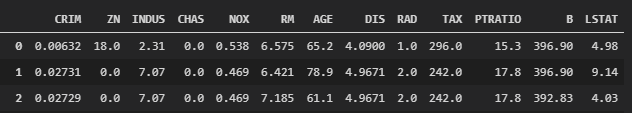
\includegraphics[width=1.0\textwidth]{abb/BostonBeispiel.PNG}
    \caption{Beispiel des Boston Datensatzes}
    \label{fig:Bild1}
\end{figure}


\subsubsection{Breast Cancer} \label{Breast Cancer}

Der \textit{Breast Cancer} Datensatz hingegen besteht aus einem binären Klassifikationsproblem.
Das bedeutet, dass das Netz nur ``ja'' oder ``nein'' kodiert als eins oder null, voraussagen
soll. Hierbei bedeutet ein Ja, dass diese Person Brustkrebs hat. Hier gibt es 
wieder einige explanatorische Variablen, die dem Netz helfen sollen zu lernen.
Diese sind Eigenschaften des Nukleus einer entommenen Brustzelle


\begin{itemize}
    \item \textbf{radius}: Radius des Nukleus
    \item \textbf{texture}: Standardabweichung der Graustufenwerte
    \item \textbf{symmetry}: Symmetrie des Nukleus
    \item \textbf{smoothness}: Lokale Abweichung der Radius Länge
\end{itemize}

Insgesamt besteht der Datensatz aus 30 solchen Variablen.

\begin{figure}[htbp] 
    \centering
       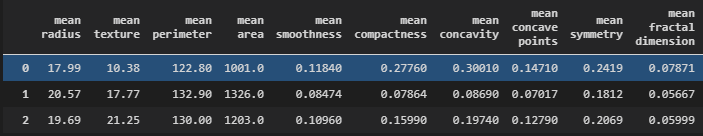
\includegraphics[width=1.0\textwidth]{abb/BreastCancerBeispiel.PNG}
    \caption{Beispiel des Breast Caner Datensatzes}
    \label{fig:Bild1}
\end{figure}

\subsection{Metrik} \label{Metrik}

Bevor wir mit dem Vergleich der verschiedenen Optimierungsmethoden der Gradienten
beginnen können, brauchen wir ein Maß für die Güte eines Ergebnisses. 
Dafür müssen wir eine Metrik definieren. Sinnvoll ist es ein neuronales Netz
daran zu messen, wieviel es richtig bewertet hat. Richtig ist im Falle des \textit{Breast Cancer}
Datensatzes einfach ob das Netz ja zu ja und nein zu nein gesagt hat. Im Falle 
des \textit{Boston House Price} Datensatzes ist richtig, wenn der Abstand vom
vorhergesagten zum echten Preis möglichst klein ist. Dies gibt uns eine 
Vielzahl von Metriken die diese Voraussetzungen erfüllen.\\

Günstiger Weise benötigen wir bereits durch das Training des neuronalen Netzes 
eine Gütefunktion die angibt ob sich die Parameter in die richtige Richtung bewegen.
Diese ist die in Abschnitt \ref{Neuronale Netze} bereits besprochene Fehlerfunktion des 
Netzes. Diese sollte unsere erste Form einer Metrik sein um das Neuronale Netz zu bewerten.

Für den \textit{Boston House Price} Datensatz ist diese Fehlerfunktion die
\textit{mittlere quadratische Abweichung}.

\begin{definition}
    \cite[S.344]{Fahrmeir.2016} Die \textbf{mittlere quadratische Abweichung} für eine Stichprobe $x_1,...,x_n$
    mit Schätzwerten $\hat{x}_1,...,\hat{x}_n$ ist definiert durch
    \begin{align}
        \frac{1}{n}\sum\limits_{i=1}^{n} (\hat{x}_i-x_i)^2
    \end{align}
\end{definition}

Dies ist die typische Fehlerfunktion für Regressionsprobleme. Man mag sich fragen
warum diese quadriert wird und nicht der absolute Abstand zum echten Wert genommen
wird, wie vorher überlegt. Diese Funktion ist aber diejenige aus der wir den Gradienten
berechnen wollen, also muss sie differenzierbar sein, was das Quadrat gewährleistet.\\

Für den \textit{Breast Cancer} Datensatz ist diese Funktion jedoch unzureichend, da 
nur null oder eins im Wertebereich der mittleren quadratischen Abweichung vorkommen würden.
Da es sich hier um ein binäres Klassifikationsproblem handelt, eignet sich die \textit{binäre Kreuzentropie}.

\begin{definition}
    \cite{Rubinstein.2004} Die \textbf{binäre Kreuzentropie} für eine Stichprobe $x_1,...,x_n$
    mit Schätzwerten $\hat{x}_1,...,\hat{x}_n$ ist definiert durch
    \begin{align}
        \frac{1}{n}\sum\limits_{i=1}^{n} x_i log(\hat{x}_i) + (1-x_i)log(1-\hat{x}_i)
    \end{align}
    wobei $log$ der natürliche Logarithmus ist.
\end{definition}

Diese Fehlerfunktion ist geeignet für Wertebereiche zwischen null und eins. Also genau 
passend für ein zwei Klassen Klassifikationsproblem. \\

Diese beiden Fehlerfunktionen geben uns eine erste Idee für die Güte des neuronalen 
Netzes und deren Prädiktion und damit auch einen Indikator, welches
Netz den besseren Optimierungsalgorithmus besitzt, wenn sonst alle Parameter 
gleich bleiben. 
Zusätzlich nehmen wir um mehr Vergleichbarkeit zu schaffen eine weitere Fehlerfunktion hinzu,
die nur der Evaluierung der besseren Optimierungsmethode dient und nicht 
für das Gradienten Abstiegsverfahren genutzt wird.
Im Falle des \textit{Boston House Price} Datensatzes benutzen wir noch den 
\textit{Mittleren absoluten Fehler}.

\begin{definition}
    Der \textbf{Mittlere absolute Fehler} für eine Stichprobe $x_1,...,x_n$
    mit Schätzwerten $\hat{x}_1,...,\hat{x}_n$ ist definiert durch
    \begin{align}
        \frac{1}{n}\sum\limits_{i=1}^{n} | \hat{x}_i-x_i |
    \end{align}
\end{definition}



\subsection{Programm und Frameworks} \label{Programm und Frameworks}



\subsection{Auswertung} \label{Auswertung}
